In folgendem Abschnitt sind die während des Versuche aufgenommenen Daten, 
so wie die aus diesen gewonnenen Ergebnisse tabellarisch und mit Hilfe 
von Grafiken dargestellt. An entsprechender Stelle werden Erklärungen zu den 
Messdaten, Rechnungen und Ergebnissen gegeben.

\subsection{Messung der mittleren Reichweite im Abstand 20mm}\label{sec:Messung_I}

	Die Messergebnisse der ersten Messung zu Bestimmung der mittleren Reichweite $R_{m}$
	sind in \cref{tab:Messwerte_I} aufgeführt. Wobei die hervorgehobene Zeile wegen der
	großen Abweichung nicht für die folgende Auswertung genutzt wurde.
	
	\begin{table}[!h]
	\centering
	\begin{tabular}{|c|c|c|c|}
		\hline
		Pos. Bild & Pos. Linse & Gegenstandsweite & Bildweite\\
		$x_{B}$ [\si{\centi\meter}] & $x_{L}$ [\si{\centi\meter}] & $g$ [\si{\centi\meter}] & $b$ [\si{\centi\meter}]\\
\hline\hline
		\num{89.6(1)} & \num{109.0(1)} & \num{20.0(1)} & \num{19.4(1)}\\
		\num{87.8(1)} & \num{104.0(1)} & \num{25.0(1)} & \num{16.2(1)}\\
		\num{84.4(1)} & \num{99.0(1)} & \num{30.0(1)} & \num{14.6(1)}\\
		\num{80.4(1)} & \num{94.0(1)} & \num{35.0(1)} & \num{13.6(1)}\\
		\num{76.0(1)} & \num{89.0(1)} & \num{40.0(1)} & \num{13.0(1)}\\
		\num{71.5(1)} & \num{84.0(1)} & \num{45.0(1)} & \num{12.5(1)}\\
		\num{66.9(1)} & \num{79.0(1)} & \num{50.0(1)} & \num{12.1(1)}\\
		\num{62.1(1)} & \num{74.0(1)} & \num{55.0(1)} & \num{11.9(1)}\\
		\num{57.2(1)} & \num{69.0(1)} & \num{60.0(1)} & \num{11.8(1)}\\
		\num{52.4(1)} & \num{64.0(1)} & \num{65.0(1)} & \num{11.6(1)}\\
		\hline
	\end{tabular}
	\caption{Gemessene Positionen des Bildes und der Linse und die daraus bestimmten 
		Bild- und Gegenstandsweiten für die Messreihe mit der bekannten Linse. Als Fehler wurde die kleinste Skaleneinteilung des
		verwendeten Millimetermaßes angenommen.  \label{tab:Auswertung_Messwerte_I}}
\end{table}

	
	In \cref{fig:Messdaten_I} sind diese Messwerte grafisch dargestellt, wobei die Gesamtzahl der gemessenen Pulse
	durch Division mit der Messdauer $t = 120 \si{s}$ in die Zerfallsrate umgerechnet wurde. 
	Die effektive Länge, die Strecke die die Alphastrahlung relativ zu Atmosphärendruck,
	zurück gelegt hat berechnet sich nach \cref{eq:effektive_laenge}.   
	
	Die mittlere Reichweite $R_{m}$ der Alphastrahlung erhält man nun, indem zunächst eine lineare 
	Regression der Messwerte durchgeführt wird. Die in \cref{fig:Messdaten_I} grau eingezeichneten Messwerte wurden 
	bei dieser Regression nicht verwendet. Mit Hilfe der Python-Bibliothek \emph{SciPy} \cite{SciPy} 
	erhält man aus den Messdaten mit dem Ansatz
	\begin{empheq}{equation}
		A(x) = a \cdot x + b,
	\end{empheq}
	die Regressionsparameter
	\addtocounter{equation}{-1}	
	\begin{subequations}
		\begin{empheq}{align}
			a &= \SI{-20(1)}{\per\second\per\milli\meter} \\
			b &= \SI{280(10)}{\per\second}.
		\end{empheq}
	\end{subequations}
	
	
	Im folgenden Schritt wird eine zur x-Achse parallele Gerade auf halber Höhe des Maximalwerts,
	der gemessenen Zerfallsraten, hier gestrichelt, eingezeichnet.\\
	 
	Die zu bestimmende Reichweite $R_{m}$ lässt sich damit als x-Koordinate des Schnittpunktes dieser beiden Geraden 
	ablesen. Die auf diese Weise ermittelte, mittlere Reichweite beträgt für diese Messdaten 
	$R_{m} = \SI{6.56(1)}{\milli\meter}$. Durch Umstellen der \cref{eq:reichweite} kann aus diesem Wert 
	die Energie der Alphastrahlung zu $E_{\alpha} = \SI{1.648(2)}{\mega\eV} $ berechnet 
	werden.\footnote{Der Fehler wurde hierbei durch \eqref{std:Energie} bestimmt.}    
	
	\begin{figure}[!h]
		\centering
		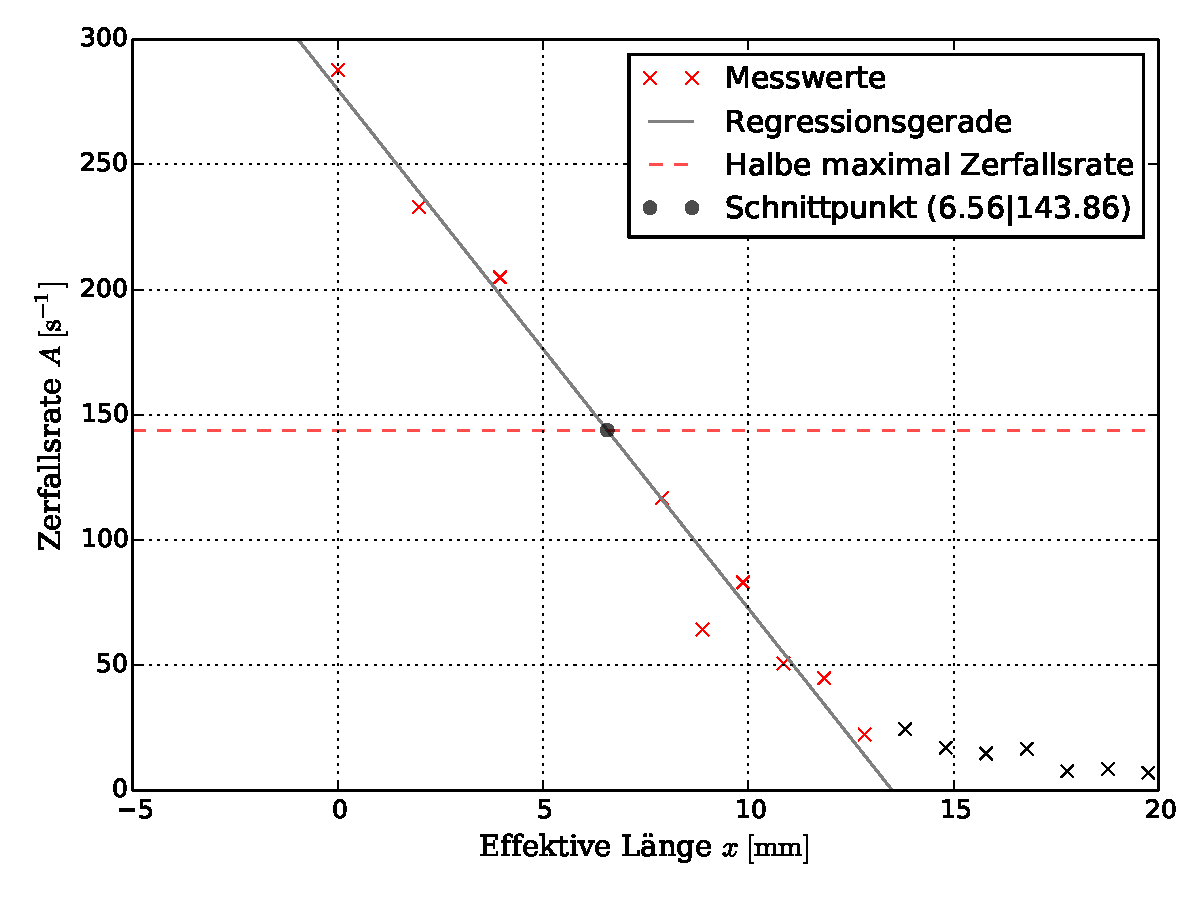
\includegraphics[scale=0.7]{Grafiken/MittlereReichweiteI.pdf}
		\caption{Darstellung der Messdaten aus \cref{tab:Messwerte_I} und Bestimmung von $R_{m}$}
		\label{fig:Messdaten_I}
	\end{figure}
	
	\vspace*{0.5cm}
	Der aus diesen Versuchsdaten zu berechnende Energieverlust $-\od{E}{x}$ wird wegen der besseren
	Messergebnisse im folgenden Unterabschnitt vorgenommen.  
	
	
\subsection{Messung der mittleren Reichweite im Abstand $25$\si{\mm}}\label{sec:Messung_II}
	
	Die bei der Messung im Abstand von \SI{25}{\milli\meter} aufgenommenen Daten sind in \cref{tab:Messwerte_II} 
	dargestellt.

	\begin{table}[!h]
	\centering
	\begin{tabular}{|c|c|c|c|c||c|}
		\hline
		Messreihe & 1 & 2 & 3 & 4 & Verschiebung\\
		Nr. &$$ & $$ & $$ & $$ & $D$ [\si{\centi\meter}]\\
\hline
\multirow{7}{1.75cm}{Ablenk-\\ strom\\$\quad\!I_{d}$\ [\si{\ampere}]}		&\num{0.00(1)} & \num{0.00(1)} & \num{0.00(1)} & \num{0.00(1)} & \num{0.0(1)}\\
		&\num{0.32(1)} & \num{0.36(1)} & \num{0.38(1)} & \num{0.38(1)} & \num{0.6(1)}\\
		&\num{0.68(1)} & \num{0.74(1)} & \num{0.82(1)} & \num{0.84(1)} & \num{1.3(1)}\\
		&\num{1.00(1)} & \num{1.10(1)} & \num{1.20(1)} & \num{1.15(1)} & \num{1.9(1)}\\
		&\num{1.30(1)} & \num{1.45(1)} & \num{1.60(1)} & \num{1.60(1)} & \num{2.5(1)}\\
		&\num{1.65(1)} & \num{1.80(1)} & \num{1.95(1)} & \num{2.00(1)} & \num{3.2(1)}\\
		&\num{2.00(1)} & \num{2.20(1)} & - & - & \num{3.8(1)}\\
		&\num{2.25(1)} & - & - & - & \num{4.4(1)}\\ \hline
\multirow{3}{1.75cm}{Beschl.\\Spannung\\$\quad\!U_{b}$\ [\si{\volt}]}	& & & & & \\
				 							   & \num{250(5)}   &   \num{300(5)}  & \num{350(5)}  & \num{400(5)} &  
				 							   \\ 
				 							   &&&&&\\\hline
		
		
		\hline
	\end{tabular}
	\caption{Messdaten zur Bestimmung des Zusammenhangs zwischen $I_d$ und $D$ \label{tab:Auswertung_Messdaten_II}}
\end{table}

		
	Wie in \cref{sec:Messung_I} beschrieben, sind auch die aus diesen Daten berechneten Zerfallsraten
	(Messzeit $ t = \SI{120}{\second}$) in \cref{fig:Messdaten_II} gegen die effektive Länge aufgetragen, um die 
	mittlere Reichweite $R_{m}$ der Alphastrahlung zu bestimmen.\\
	Die dafür notwendige lineare Regression mit dem Ansatz
	\begin{empheq}{equation}
		A(x) = c \cdot x + d, 
	\end{empheq}
	ergibt die Regressionsparameter 
	\addtocounter{equation}{-1}
	\begin{subequations}
		\begin{empheq}{align}
			c &= \SI{-15.2(9)}{\per\second\per\milli\meter}\\
			d &= \SI{271(12)}{\per\second}.
		\end{empheq}
	\end{subequations}
	Aus diesen Daten ergibt sich die mittlere Reichweite von $R_{m} = \SI{8.39(1)}{\milli\meter}$.
	Auch aus diesem Wert lässt sich durch Umstellen der \cref{eq:reichweite} die Energie der 
	Alphastrahlung zu $E_{\alpha} = \SI{1.943(2)}{\mega\eV} $ bestimmen.
	\footnote{Der Fehler wurde hierbei durch \cref{std:Energie} bestimmt.} 
	
	\begin{figure}[!h]
		\centering
		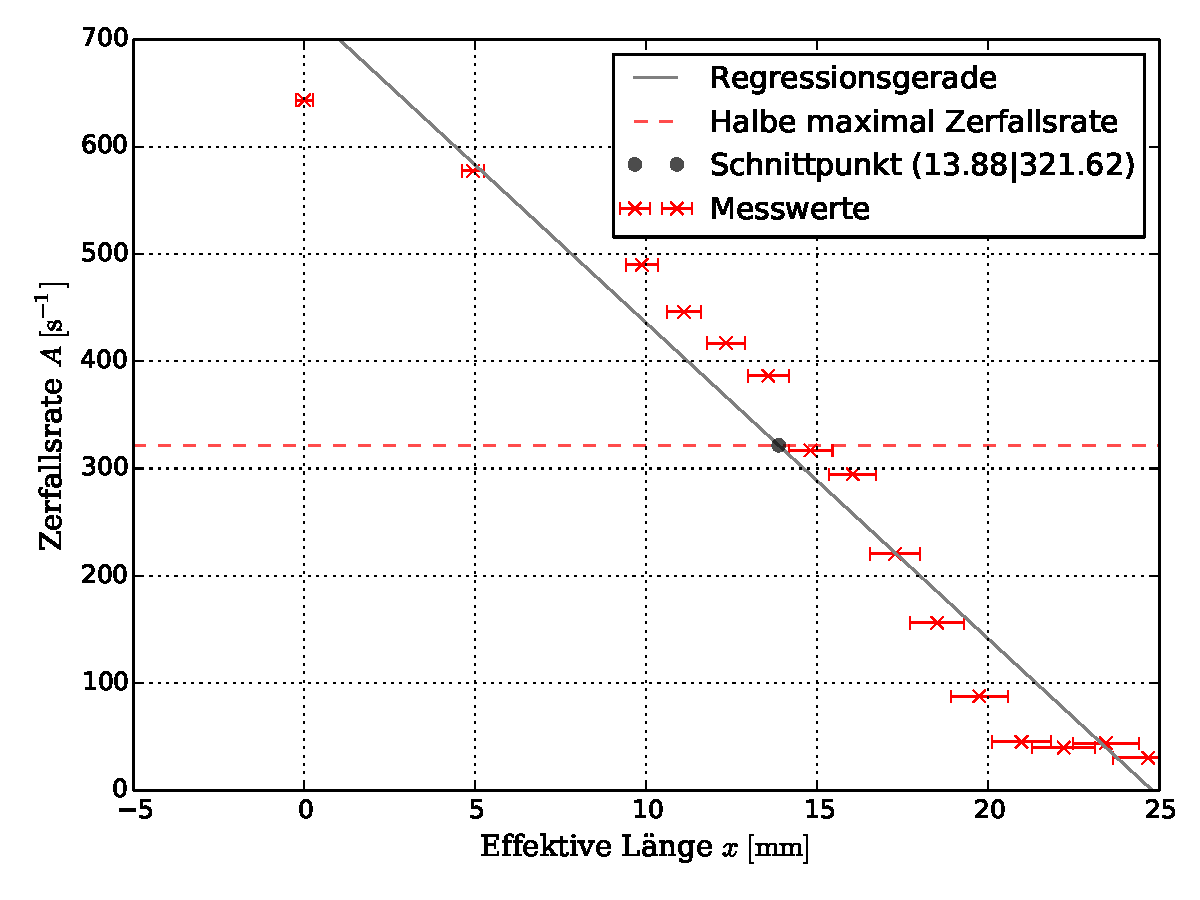
\includegraphics[scale=0.7]{Grafiken/MittlereReichweiteII.pdf}
		\caption{Darstellung der Messdaten aus \cref{tab:Messwerte_II} und Bestimmung von $R_{m}$}
		\label{fig:Messdaten_II}
	\end{figure}

	Durch das Auftragen der maximal Energien $E_{max}$ aus \cref{tab:Messwerte_II} gegen die effektive Länge $x$,
	in \cref{fig:Messdaten_II_Energie}, ist es möglich mit einem der Bethe-Bloch-Gleichung \cref{eq:bethe-bloch} 
	ähnlichen Regressionsansatz 
	\begin{empheq}{equation}
		E(x) = e \cdot \Ln{f \cdot x}, 
	\end{empheq}
	die Funktion des Energieverlaufs mit den Regressionsparametern
	\addtocounter{equation}{-1}
	\begin{subequations}
		\begin{empheq}{align}
			e &= \SI{-0.42(6)}{\mega\eV}\\
			f &= \SI{4(4)e-05}{\per\milli\meter}
		\end{empheq}
	\end{subequations}	
	zu bestimmen.\\
	Durch Differentiation der auf diese Weise bestimmten Funktion $E(x)$ erhält man die gesuchte Energieänderung
	$\od{E}{x} = \frac{e}{x}  = \frac{\num{-0.42}}{x} \si{\mega\eV\per\milli\meter} $ und daraus der Energieverlust 
	$-\od{E}{x} = \frac{\num{0.42}}{x} \si{\mega\eV\per\milli\meter}$.

	\begin{figure}[!h]
		\centering
		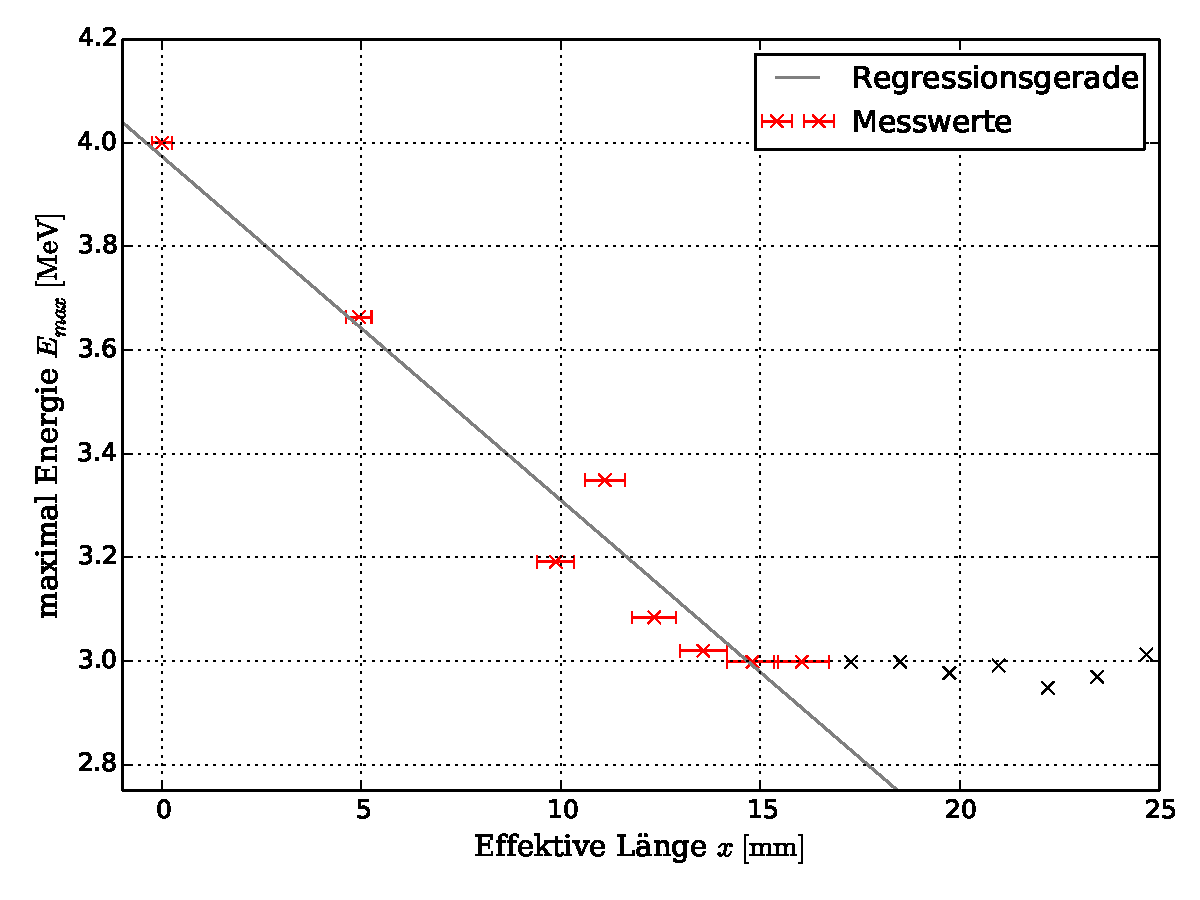
\includegraphics[scale=0.7]{Grafiken/EnergieVerlauf.pdf}
		\caption{Darstellung der maximal Energie in Abhängigkeit der effektiven Länge}
		\label{fig:Messdaten_II_Energie}
	\end{figure}
	

\subsection{Statistik des radioaktiven Zerfalls}\label{sec:Messung_III}
	
	In \cref{tab:Messwerte_III} sind die  während der Messzeit 
	$\Delta t = \SI{10}{\second}$ aufgenommenen Zerfallsraten aufgelistet.
	\begin{table}[!h]
	\centering
	\begin{tabular}{|c|c|}
		\hline
		Versuch Nr. & Anzahl Pulse\\
\hline\hline
		\num{1} & \num{569}\\
		\num{2} & \num{616}\\
		\num{3} & \num{590}\\
		\num{4} & \num{566}\\
		\num{5} & \num{599}\\
		\num{6} & \num{627}\\
		\num{7} & \num{612}\\
		\num{8} & \num{604}\\
		\num{9} & \num{596}\\
		\num{10} & \num{618}\\
		\num{11} & \num{617}\\
		\num{12} & \num{621}\\
		\num{13} & \num{634}\\
		\num{14} & \num{603}\\
		\num{15} & \num{588}\\
		\num{16} & \num{669}\\
		\num{17} & \num{633}\\
		\num{18} & \num{630}\\
		\num{19} & \num{618}\\
		\num{20} & \num{590}\\
		\num{21} & \num{593}\\
		\num{22} & \num{595}\\
		\num{23} & \num{575}\\
		\num{24} & \num{600}\\
		\num{25} & \num{682}\\
		\num{26} & \num{636}\\
		\num{27} & \num{639}\\
		\num{28} & \num{670}\\
		\num{29} & \num{601}\\
		\num{30} & \num{628}\\
		\num{31} & \num{652}\\
		\num{32} & \num{599}\\
		\num{33} & \num{663}\\
		\num{34} & \num{617}\\
		\num{35} & \num{1223}\\
		\num{36} & \num{1308}\\
		\num{37} & \num{841}\\
		\num{38} & \num{647}\\
		\num{39} & \num{598}\\
		\num{40} & \num{633}\\
		\num{41} & \num{645}\\
		\num{42} & \num{593}\\
		\num{43} & \num{573}\\
		\num{44} & \num{603}\\
		\num{45} & \num{561}\\
		\num{46} & \num{645}\\
		\num{47} & \num{611}\\
		\num{48} & \num{575}\\
		\num{49} & \num{590}\\
		\num{50} & \num{591}\\
		\num{51} & \num{692}\\
		\num{52} & \num{601}\\
		\num{53} & \num{655}\\
		\num{54} & \num{776}\\
		\num{55} & \num{783}\\
		\num{56} & \num{997}\\
		\num{57} & \num{838}\\
		\num{58} & \num{683}\\
		\num{59} & \num{681}\\
		\num{60} & \num{815}\\
		\num{61} & \num{628}\\
		\num{62} & \num{670}\\
		\num{63} & \num{652}\\
		\num{64} & \num{623}\\
		\num{65} & \num{620}\\
		\num{66} & \num{719}\\
		\num{67} & \num{858}\\
		\num{68} & \num{597}\\
		\num{69} & \num{658}\\
		\num{70} & \num{638}\\
		\num{71} & \num{649}\\
		\num{72} & \num{688}\\
		\num{73} & \num{707}\\
		\num{74} & \num{896}\\
		\num{75} & \num{844}\\
		\num{76} & \num{593}\\
		\num{77} & \num{746}\\
		\num{78} & \num{1089}\\
		\num{79} & \num{674}\\
		\num{80} & \num{754}\\
		\num{81} & \num{750}\\
		\num{82} & \num{834}\\
		\num{83} & \num{795}\\
		\num{84} & \num{703}\\
		\num{85} & \num{858}\\
		\num{86} & \num{702}\\
		\num{87} & \num{636}\\
		\num{88} & \num{599}\\
		\num{89} & \num{1206}\\
		\num{90} & \num{664}\\
		\num{91} & \num{609}\\
		\num{92} & \num{660}\\
		\num{93} & \num{662}\\
		\num{94} & \num{663}\\
		\num{95} & \num{689}\\
		\num{96} & \num{644}\\
		\num{97} & \num{648}\\
		\num{98} & \num{604}\\
		\num{99} & \num{613}\\
		\num{100} & \num{581}\\
		\hline
	\end{tabular}
	\caption{Anzahl der gemessenen Impulse \label{tab:Messwerte_III}}
\end{table}

	Der Mittelwert und die Standardabweichung dieser Messwerte berechnen sich zu
	\begin{empheq}{align}
		\mean{A} &= \SI{681(14)}{\per\second}\\
		\sigma_{A} &= \SI{136}{\per\second}\\
	\end{empheq}
	
	Diese Messwert sind in \cref{fig:Messdaten_III} in einem Histogramm aufgetragen,
	in dem die Balkenbreite $\Delta N = \SI{20}{\per\second}$ gewählt wurde.
	
	In den Abbildungen \ref{fig:Messdaten_III_Poisson} und \ref{fig:Messdaten_III_Gauss}
	ist das Histogramm aus \cref{fig:Messdaten_III} noch einmal im Vergleich zu einer 
	diskreten Poisson- bzw. kontinuierlichen Gauß-Verteilung mit dem Mittelwert der 
	Messdaten dargestellt.
	
	
	\begin{figure}[!h]
		\centering
		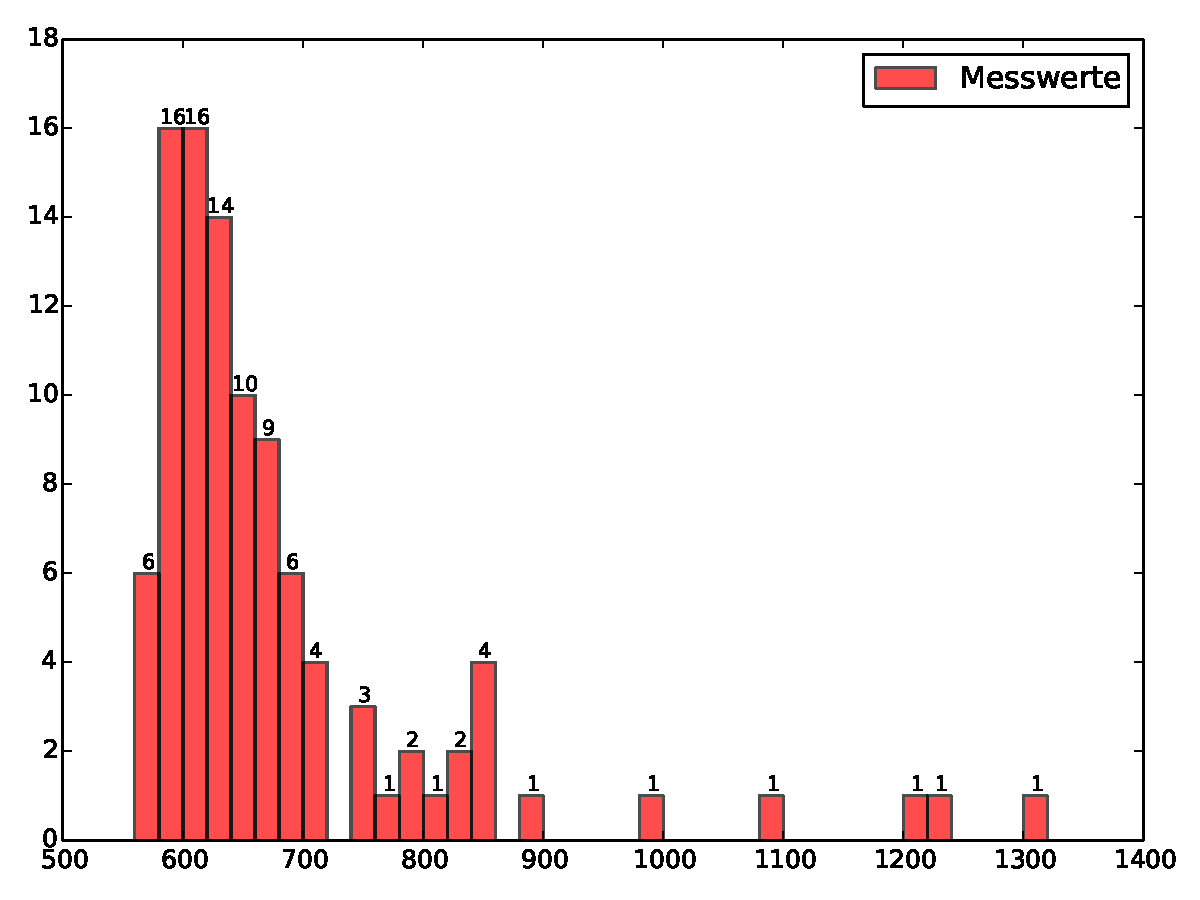
\includegraphics[scale=0.7]{Grafiken/AktivitaetHistogramm.pdf}
		\caption{Darstellung der Messdaten aus \cref{tab:Messwerte_II} und Bestimmung von $R_{m}$}
		\label{fig:Messdaten_III}
	\end{figure}
		
	\begin{figure}[!h]
		\centering
		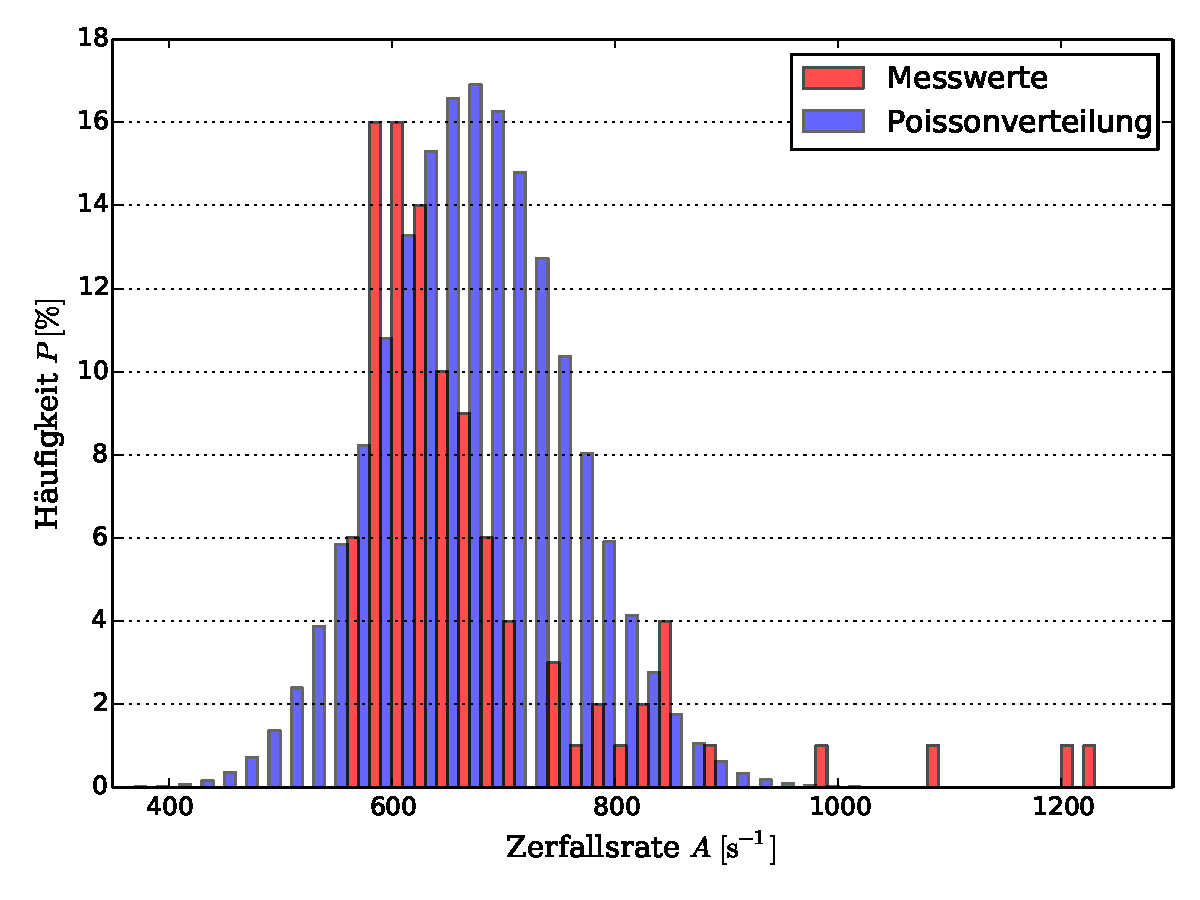
\includegraphics[scale=0.7]{Grafiken/VergleichPoisson.pdf}
		\caption{Vergleiche der Messdaten mit der diskreten Poissonverteilung}
		\label{fig:Messdaten_III_Poisson}
	\end{figure}
	
	\begin{figure}[!h]
		\centering
		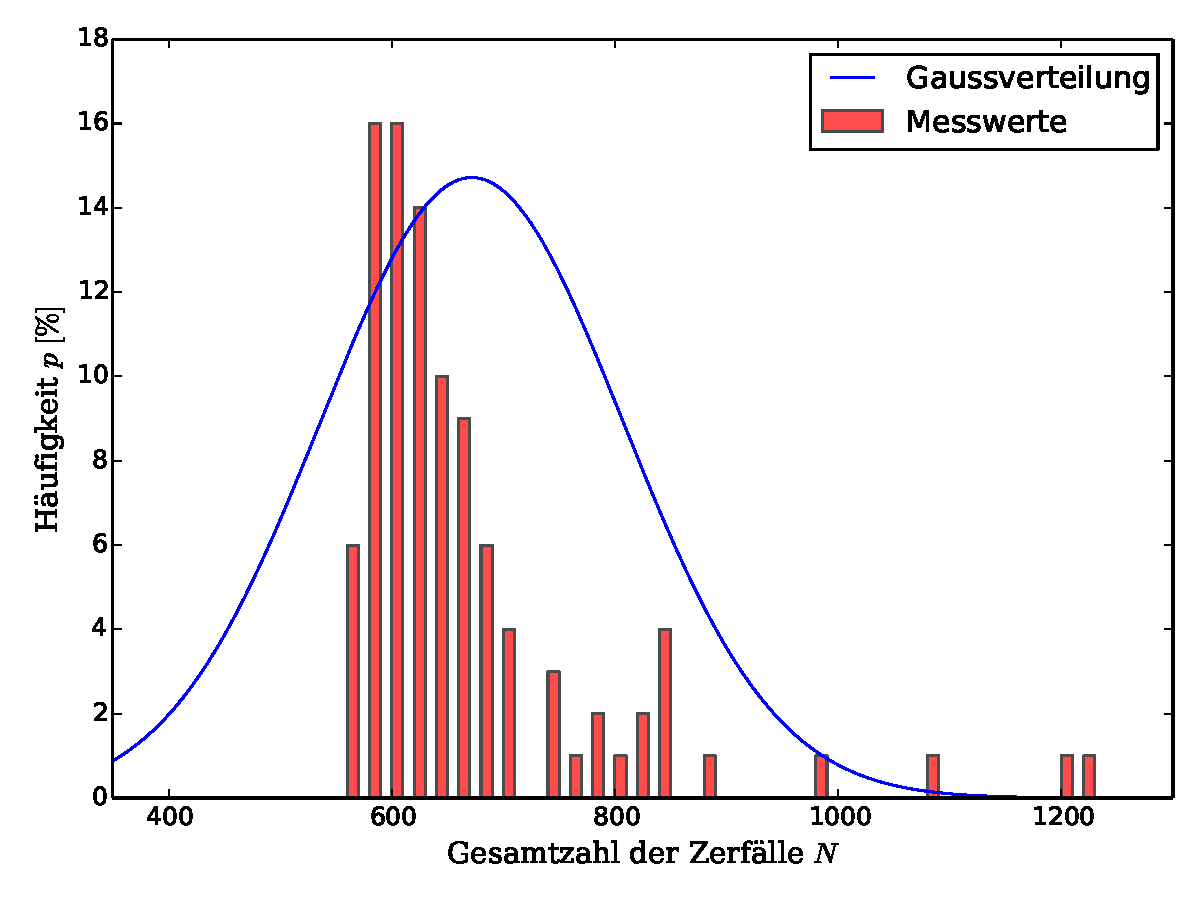
\includegraphics[scale=0.7]{Grafiken/VergleichGauss.pdf}
		\caption{Vergleich der Messdaten mit der kontinuierlichen Gaussverteilung}
		\label{fig:Messdaten_III_Gauss}
	\end{figure}
